%%%%%%%%%%%%%%%%%%%%%%%%%%%%%%%%%%%%%%%%%%%%%%%%%%%%%%%%%%%%%%%%%%%%%
%% This is a (brief) model paper using the achemso class
%% The document class accepts keyval options, which should include
%% the target journal and optionally the manuscript type. 
%%%%%%%%%%%%%%%%%%%%%%%%%%%%%%%%%%%%%%%%%%%%%%%%%%%%%%%%%%%%%%%%%%%%%
\documentclass[journal=jacsat,manuscript=article]{achemso}

%%%%%%%%%%%%%%%%%%%%%%%%%%%%%%%%%%%%%%%%%%%%%%%%%%%%%%%%%%%%%%%%%%%%%
%% Place any additional packages needed here.  Only include packages
%% which are essential, to avoid problems later. Do NOT use any
%% packages which require e-TeX (for example etoolbox): the e-TeX
%% extensions are not currently available on the ACS conversion
%% servers.
%%%%%%%%%%%%%%%%%%%%%%%%%%%%%%%%%%%%%%%%%%%%%%%%%%%%%%%%%%%%%%%%%%%%%
\usepackage[version=3]{mhchem} % Formula subscripts using \ce{}
\usepackage{color}
\usepackage{xcolor}

%%%%%%%%%%%%%%%%%%%%%%%%%%%%%%%%%%%%%%%%%%%%%%%%%%%%%%%%%%%%%%%%%%%%%
%% If issues arise when submitting your manuscript, you may want to
%% un-comment the next line.  This provides information on the
%% version of every file you have used.
%%%%%%%%%%%%%%%%%%%%%%%%%%%%%%%%%%%%%%%%%%%%%%%%%%%%%%%%%%%%%%%%%%%%%
%%\listfiles

%%%%%%%%%%%%%%%%%%%%%%%%%%%%%%%%%%%%%%%%%%%%%%%%%%%%%%%%%%%%%%%%%%%%%
%% Place any additional macros here.  Please use \newcommand* where
%% possible, and avoid layout-changing macros (which are not used
%% when typesetting).
%%%%%%%%%%%%%%%%%%%%%%%%%%%%%%%%%%%%%%%%%%%%%%%%%%%%%%%%%%%%%%%%%%%%%
\newcommand*\mycommand[1]{\texttt{\emph{#1}}}
\def\selrev#1{\textcolor{blue}{#1}}

%%%%%%%%%%%%%%%%%%%%%%%%%%%%%%%%%%%%%%%%%%%%%%%%%%%%%%%%%%%%%%%%%%%%%
%% Meta-data block
%% ---------------
%% Each author should be given as a separate \author command.
%%
%% Corresponding authors should have an e-mail given after the author
%% name as an \email command. Phone and fax numbers can be given
%% using \phone and \fax, respectively; this information is optional.
%%
%% The affiliation of authors is given after the authors; each
%% \affiliation command applies to all preceding authors not already
%% assigned an affiliation.
%%
%% The affiliation takes an option argument for the short name.  This
%% will typically be something like "University of Somewhere".
%%
%% The \altaffiliation macro should be used for new address, etc.
%% On the other hand, \alsoaffiliation is used on a per author basis
%% when authors are associated with multiple institutions.
%%%%%%%%%%%%%%%%%%%%%%%%%%%%%%%%%%%%%%%%%%%%%%%%%%%%%%%%%%%%%%%%%%%%%
\author{Sélène Forget}
\affiliation[ENS]
{CPCV, Département de Chimie, École Normale Supérieure, PSL University, Sorbonne University, CNRS, 75005 Paris}
\email{selene.forget@ens.psl.eu}
\author{I. Ken Groupleader}
\email{guillaume.stirnemann@ens.psl.eu}
\affiliation[ENS]
{CPCV, Département de Chimie, École Normale Supérieure, PSL University, Sorbonne University, CNRS, 75005 Paris}



%%%%%%%%%%%%%%%%%%%%%%%%%%%%%%%%%%%%%%%%%%%%%%%%%%%%%%%%%%%%%%%%%%%%%
%% The document title should be given as usual. Some journals require
%% a running title from the author: this should be supplied as an
%% optional argument to \title.
%%%%%%%%%%%%%%%%%%%%%%%%%%%%%%%%%%%%%%%%%%%%%%%%%%%%%%%%%%%%%%%%%%%%%
\title[An \textsf{achemso} demo]
  {Molecular Dissection of Hairpin Ribozyme Catalyzed Self-Cleavage}

%%%%%%%%%%%%%%%%%%%%%%%%%%%%%%%%%%%%%%%%%%%%%%%%%%%%%%%%%%%%%%%%%%%%%
%% Some journals require a list of abbreviations or keywords to be
%% supplied. These should be set up here, and will be printed after
%% the title and author information, if needed.
%%%%%%%%%%%%%%%%%%%%%%%%%%%%%%%%%%%%%%%%%%%%%%%%%%%%%%%%%%%%%%%%%%%%%
\abbreviations{IR,NMR,UV}
\keywords{American Chemical Society, \LaTeX}

%%%%%%%%%%%%%%%%%%%%%%%%%%%%%%%%%%%%%%%%%%%%%%%%%%%%%%%%%%%%%%%%%%%%%
%% The manuscript does not need to include \maketitle, which is
%% executed automatically.
%%%%%%%%%%%%%%%%%%%%%%%%%%%%%%%%%%%%%%%%%%%%%%%%%%%%%%%%%%%%%%%%%%%%%
\begin{document}

%%%%%%%%%%%%%%%%%%%%%%%%%%%%%%%%%%%%%%%%%%%%%%%%%%%%%%%%%%%%%%%%%%%%%
%% The "tocentry" environment can be used to create an entry for the
%% graphical table of contents. It is given here as some journals
%% require that it is printed as part of the abstract page. It will
%% be automatically moved as appropriate.
%%%%%%%%%%%%%%%%%%%%%%%%%%%%%%%%%%%%%%%%%%%%%%%%%%%%%%%%%%%%%%%%%%%%%
\begin{tocentry}

Some journals require a graphical entry for the Table of Contents.
This should be laid out ``print ready'' so that the sizing of the
text is correct.

Inside the \texttt{tocentry} environment, the font used is Helvetica
8\,pt, as required by \emph{Journal of the American Chemical
Society}.

The surrounding frame is 9\,cm by 3.5\,cm, which is the maximum
permitted for  \emph{Journal of the American Chemical Society}
graphical table of content entries. The box will not resize if the
content is too big: instead it will overflow the edge of the box.

This box and the associated title will always be printed on a
separate page at the end of the document.

\end{tocentry}

%%%%%%%%%%%%%%%%%%%%%%%%%%%%%%%%%%%%%%%%%%%%%%%%%%%%%%%%%%%%%%%%%%%%%
%% The abstract environment will automatically gobble the contents
%% if an abstract is not used by the target journal.
%%%%%%%%%%%%%%%%%%%%%%%%%%%%%%%%%%%%%%%%%%%%%%%%%%%%%%%%%%%%%%%%%%%%%
\begin{abstract}
[...]
\end{abstract}

%%%%%%%%%%%%%%%%%%%%%%%%%%%%%%%%%%%%%%%%%%%%%%%%%%%%%%%%%%%%%%%%%%%%%
%% Start the main part of the manuscript here.
%%%%%%%%%%%%%%%%%%%%%%%%%%%%%%%%%%%%%%%%%%%%%%%%%%%%%%%%%%%%%%%%%%%%%
\section{Introduction}
The discovery of catalytic RNAs, or ribozymes, have drastically changed our view of biological catalysis, 
proving that cell activity can be undertaken by more than proteins. 
Yet the full comprehension of the chemistry at play in these systems remains uncertain, 
with notably remaining debates on how mechanistically does the catalyst perform the reaction. 
\selrev{Ettoffer un peu ici. Peut être faire un petit inventaire de ce que l'on connait des autres ryb ?}

Among the most-studied ribozymes outstands the hairpin ribozyme (HpR), which performs the cleavage of a phosphodiester bond upon its own backbone,
with a 3'-5' polymeric linkage of its nucleic backbone replaced by a 2'-3' cyclic terminating linkage.  
The HpR is not the only ribozyme to be self-reactive, but it was found to be one of the few to be able to do so without requiring any ion. 
% Enjeu globau : mais commentles ARNs s'y prennent ils ? Prendre un example d'itérêt : sans ion, reaction de self-cleavage du HpR.
% Pourquoi est il difficile de trancher le débat ? Object auto reactif difficile à étudier expérimentalement
%% Du coup on peut faire de la simulation a partir des structures dont l'ont dispose mais pas facile de tracnher le débat car objet très flexibles
%Additionally, and despite being characterized as a self-cleaving specie, its chemical equilibrium is rather in favor of ligation.
If we do have proof that all chemical components involved in the self-splicing reaction are part of the RNA itself, we do not 
know exactly which RNA atoms take part, and neither do we know how exactly do they proceed the self-cleavage. 

% MECHANISTIC PRESENTATION 
%% Argument pro and cons for each ?
%% Opposition between insights from simulation and experiment
In this transphosphoesterification process, 
the central step is an addition-elimination step, which involved the formation of a pentavalent phosphorus transition state.
For this to occur, two key questions arise: how is the nucleophilic group activated prior to the addition step?
And how is the departing group activated prior to the elimination step?

Mutagenesis experiments \cite{kuzmin_role_2005}, reinforced by structural resolution studies \cite{rupert_crystal_2001,salter_water_2006},
have demonstrated that two surrounding nucleobases, G8 and A38, are (i) mandatory for the chemical activity and (ii) in the direct neighbourhood of the A-1 --- G+1 junction.
From there, a first mechanistic scenarios was proposed: the dianionic scenario proposes that both G8 and A38 are directly involved, 
acting respectively as the general base that activates the nucleophile O2' by capturing its proton, 
and as the general acid that reprotonates the leaving group O5' after the elimination step (see Figure \ref{fig:all_mecas} A).
Despite supporting pH-dependency experiments, this cleavage scenario suffers from one major inconsistency, 
which is the necessary prior deprotonation but \textit{in-vivo} impractical of the N1 atom of G8 nucleobase.

To address this insufficiency, a second scenario has been considered: the in-line monoanionic scenario (see Figure \ref{fig:all_mecas} B). 
Here, A38 and G8 nucleobases only contribute to the electrostatic stabilization of the transition state, 
being involved in several H-bonds with atoms of the scissible junction. 
En more, these non-covalent interactions force the catalytic site to arrange favorably for the initiation of the reaction.
While being maintained in position, 
the deprotonation of the O2' atom of A-1 is performed by one of the non-bridging oxygens the phosphate group itself, 
leading to a monoprotic phosphate intermediate. 
However, this scenario also suffers from its apparent incompatibility with the experimental pH-dependency of the reaction, 
as argued by Kath-Schorr et al. \cite{kath-schorr_general_2012}.

All this debate remains unsettled so far because of the inherent self-reactiveness of the HpR. 
Indeed, because it is self-reactive, the hairpin ribozyme can not be structurally resolved in directly as such.
Instead, mimics of the HpR in wich the chemical activity is inhibited, etiher by removing the O2' oxygen nuclophilr, by methylating it
or by replacing other chemical groups with non-reactive ones, are used to study the catalytic site.
Thus, no one can directly observe the catalytic site in its reactive form.
With arguments based on crystal structures of \textit{mimics} of the catalytic states,
and non-discriminative pH profiles, it has been hard to draw definitive conclusions from experiments only.

In parallel to the experimental efforts, the HpR has been studied using \textit{in silico} tools.
Complementary to X-ray crystal studies, molecular dynamics (MD) expands the knowledge gained through structural resolution
by providing the dynamic behavior of the resolved object. 
Here, the challenge of studying self-reactive objects is no longer a problem,
as one can simulate any reactive species without worrying about self-degradation.
These studies aimed at studying two aspects : first, the conformational landscape of the HpR, from extanded simulation of the full HpR with classical force fields \cite{mlynsky_extensive_2010, mlynsky_reactive_2015,kumar_mechanistic_2018},
and second, the chemical activity itself, with mixed quantic and classic mechanics (QM/MM) simulations \cite{mlynsky_qmmm_2011, mlynsky_comparison_2014, mlynsky_qmmm_2011, nam_electrostatic_2008, nam_electrostatic_2009,kumar_deciphering_2020}.
Far from discriminating a mechanistic route over the other, these studies rather support the idea of potentially coexistent mechanistic strategies.

Anyway, they suffer from the inherent limitations of MD: on one hand the lack of accuracy in of the classical force fields,
and on the other hand the limited conformational sampling of QM/MM simulations.





%% Pas de simulation de l'état clivé encore 
All we have is the knowledge that the ribozyme is self-reactive and can perform the cleavage without any cofactor. We are missing simulations of the cleaved states, which are necessary to understand the chemical activity of the ribozyme.
fill the partial knwoledge led us to concieve ..

Althought 
The simulation will provide relevant structures of either reactive, product, or transition states,
which are mandatory for subsequent quantum calculations.


\begin{figure}[h]
  \centering
  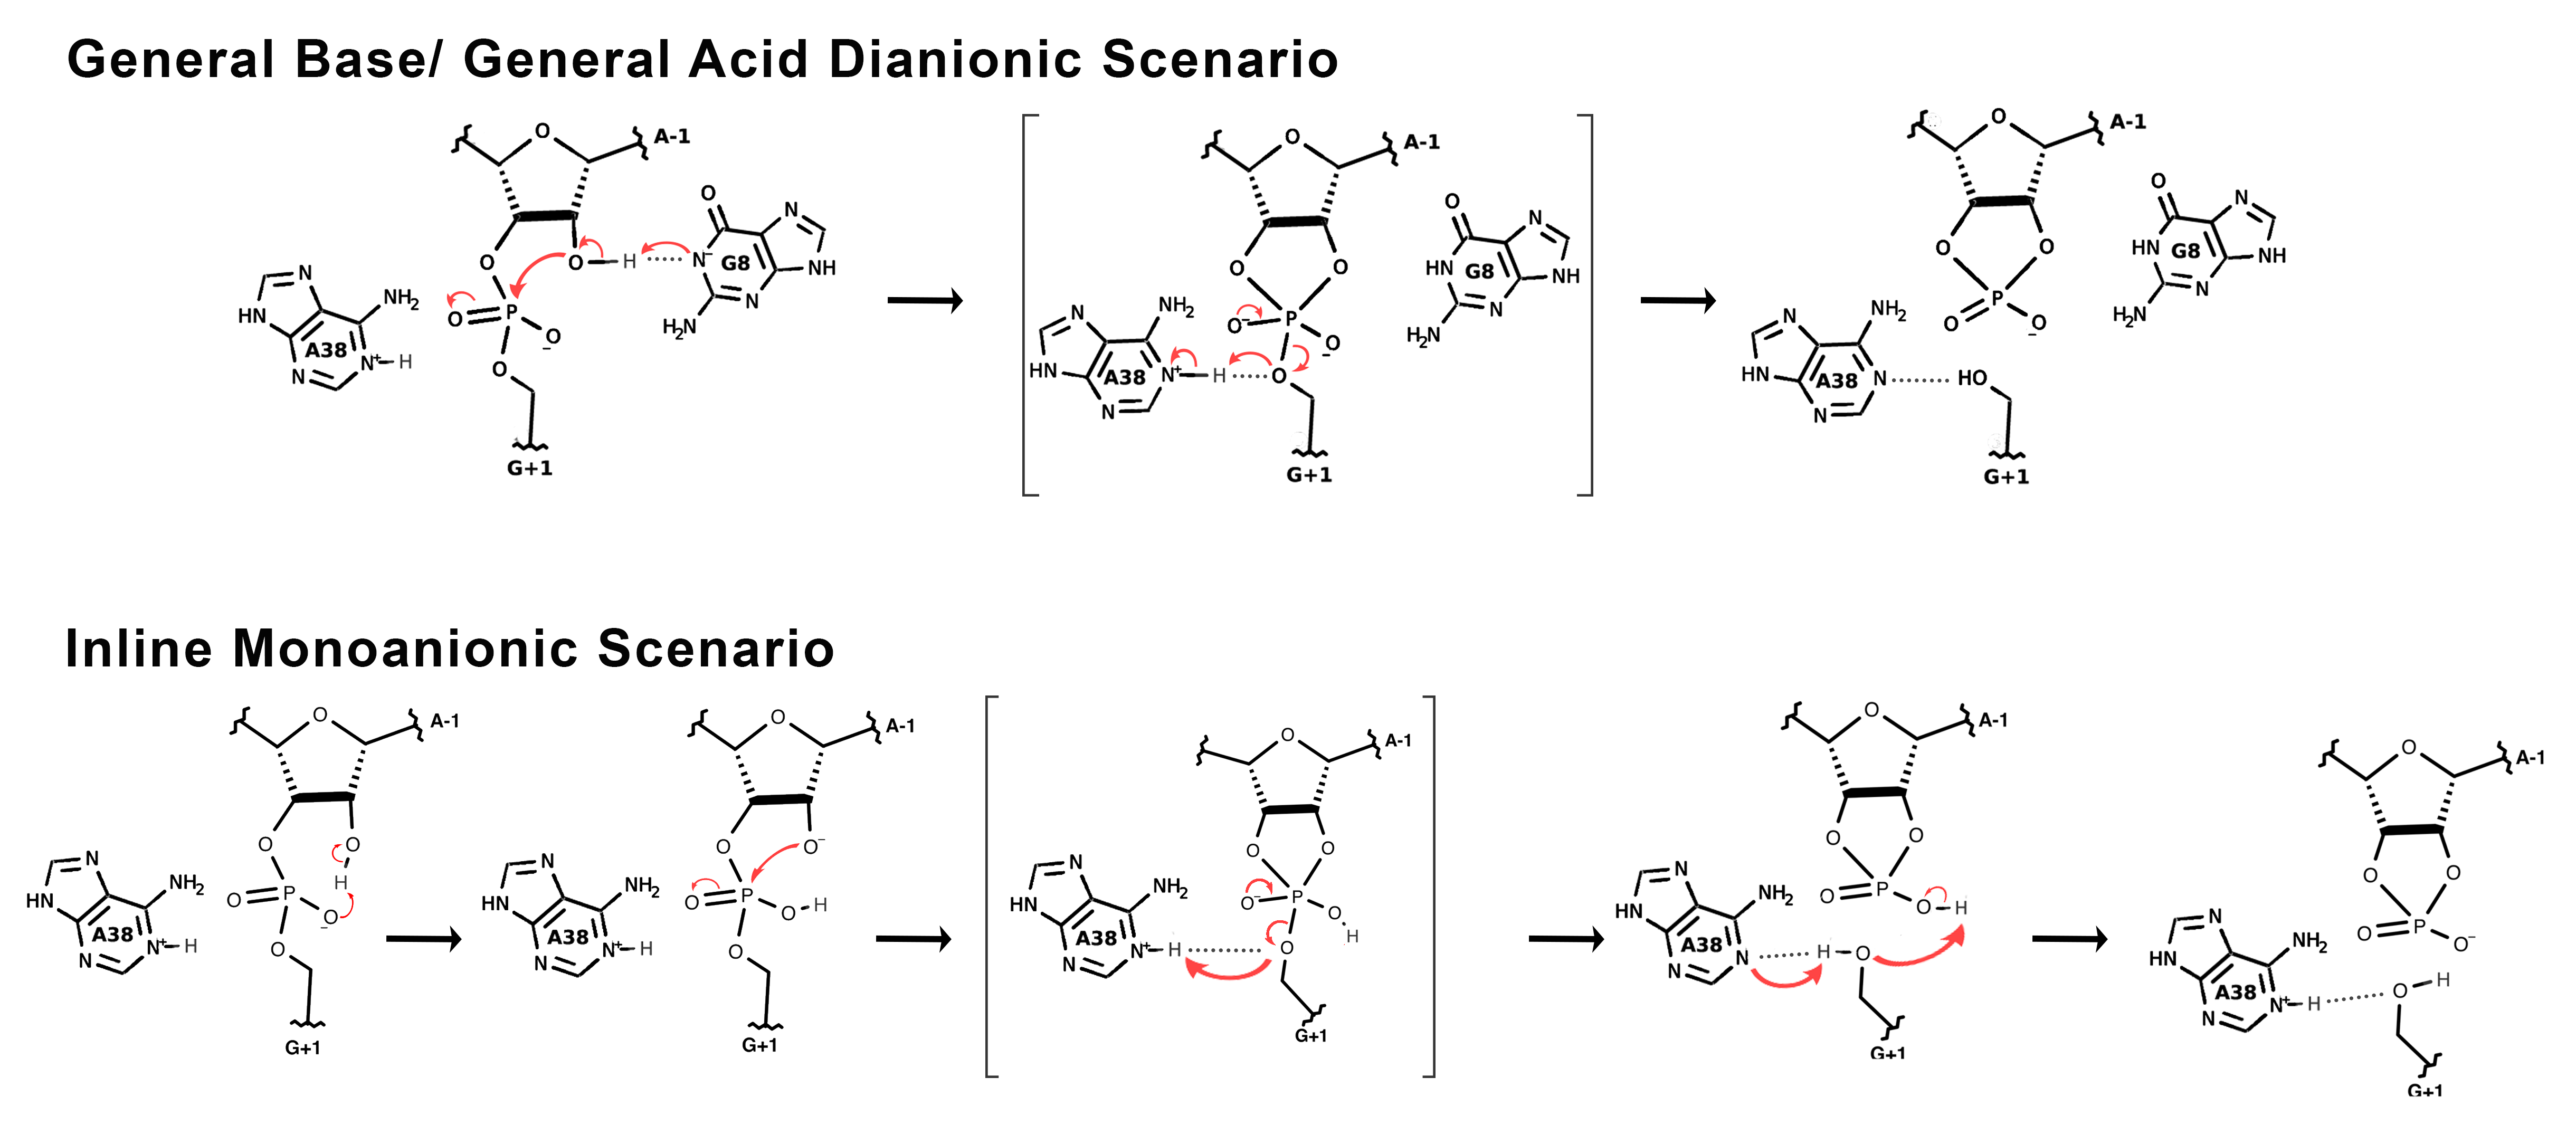
\includegraphics[width=\textwidth]{figures/All_mecanisms.png}
  \caption[Mechanistic Pathways of the Self-Cleavage]
  {Detailed schemes of the three proposed mechanisms for the Hairpin Ribozyme self-cleavage reaction:
  the general acid-base mechanism, the inline mono-anionic mechanism, and the A38 mediated proton shuttle scenario.
  We chose here to represent the inline mono-anionic mechanism with the A38 mediated proton transfer in the elimination step. 
  The direct reprotonation of O5' by the phosphate group is shown in Figure \ref{fig:monoanionic_general} in chapter \ref{chap:hpR_mechanism}.}
  \label{fig:all_mecas}
\end{figure}



% Enumeration de notre plan.

In this study, we provide insights to the mechanistic debate by investigating the conformational landscape of different "intermediates".
We 



% Résultats partiels. 



%%%%%%%%%%%%%%%%%%%%%%%%%%%%%%%%%
\section{Materials and Methods}

\subsection{Simulation of the HpR intermediates and Analysis Softwares}

The different simulations of the hairpin ribozyme intermediates were performed using the GROMACS 2022.3 \cite{abraham_gromacs_2015} patched with PLUMED 2.7 \cite{tribello_plumed_2014, the_plumed_consortium_promoting_2019}.
The visualization and analysis of the REST2 trajectories were performed using respectively 
\paragraph{Simulation of Product States}
The initial structures of all the cleaved states investigated in this study were constructed
from the crystallographic structure of the 61-mer minimal hairpin ribozyme resolved at 2.2 \AA,
in which the G+1 phosphate group was removed (PDB ID: 2P7D, see Table \ref{tab:hpR_crystals}) \cite{torelli_comparison_2007}.
The missing phosphate (P, Opro-Rp, Opro-Sp atoms) was positioned according to the Vanadate Structure (PDB ID: 2P7E).
After superposing the respective A-1 nucleotides, 
the Cartesian coordinates of the vanadate were extracted to be used for the phosphorus atom, and the same goes for the oxygen atoms.\\
Additionally, a conformational heterogeneity at nucleobase G8 in the cleaved product mimic crystal structure was observed, 
with 50\% of the population with G8 in the syn conformation, 50\% in the anti conformation \cite{torelli_comparison_2007}.
Both conformations were reported in the crystal structure. 
We chose to keep the anti conformer, as this is the conformation of the ligated structure, 
the most populated conformer of the vanadate transition state mimic (PDB ID: 2P7E), 
and the one that was resolved in the pre-catalytic state (PDB ID: 2OUE) and in the product state of the 4WJ ribozyme (PDB ID: 1M5K).

The positions of the final catalytic site atoms (in the crystal structure) were compared to the 4WJ cleaved HpR equivalent (PDB ID: 1M5V)
and demonstrated excellent consistency, with an RMSD of 0.93~\AA\ calculated over all heavy atoms of residues A-1, G+1, G8 and A38 (see Figure \ref{fig:cleaved_crystals}).


\paragraph{Forcefields.}

\paragraph{Preparation of Non-Standard Residues.}

The intermediates of the hairpin ribozyme with the most probable protonation states of the (isolated)
chemical groups at \textit{in vivo} pH.
The existing force fields do not include the parameters for these non-standard states, 
which need to be generated specifically for this purpose.
There are three possible situations:



\subsection{Descriptors.}


Similarly to the ligated states, 
the analysis of the cleaved catalytic site implies the monitoring of certain key variables, 
chosen for the relevancy regarding the mechanism.
Here, we focus on to following observables: 
\begin{itemize}
    \item IAA and d$_\mathrm{G+1:O5' - A-1:PC}$ which are the key observables for the nucleophilic attack,
    \item d$_\mathrm{A-1:O2' - G8:N1}$, d$_\mathrm{A-1:O2' - A38:N6}$,d$_\mathrm{OproSp - G8:N2}$, d$_\mathrm{OproRp - G8:N2}$, which informs on the positions of surrounding A38 and G8 regarding the 3' termini strand.
    \item d$_\mathrm{G+1:O5' - A38:N1}$ which informs on the role of A38 in the proton transfer.
    \item d$_\mathrm{OproSp - G+1:O5'}$, d$_\mathrm{OproRp - G+1:O5'}$ which informs on the variant of the inline scenario proton transfer.
    \item The puckering of the G+1 ribose, symmetrically to A-1.
\end{itemize}
% The same combination analysis as the one done over the ligated pre-catalytic state (detailed in Chapter \ref{chap:minimal}) 
% has been conducted here, but using these cleavaed-state key observables.
% By analogy, we refer to this analysis as the 10-key observables combination analysis.

\subsection{Convergence.}
In the ligated state, convergence was established using both the eRMSD as global metric
 and conformational labeling described above as local metric.
Figure \ref{fig:Int_REST2_Convergence} A-D details the time evolution of these metrics for the ligated states.
In the cleaved state, we did not settle any satisfying local collective variable, and had to rely on the eRMSD global metric only 
(see Figure\ref{fig:Int_REST2_Convergence} E-F).



%%%%%%%%%%%%%%%%%%%%
\section{Results}

Althought unrelevant scientifically speaking, 
we choose here to consider accordingly every species that could appear along the different mechanistic pathways, 
starting with the mono-anionic scenario. 

\subsection{Mono-Anionic Scenario}

The mono-anionic mechanism begins with a proton transfer from the O2' to one of the two oxygens of the scissile phosphate,
leading to the formation of the "AP" intermediate (see Figure \ref{fig:monoanionic_general}).
From there, the deprotonated O2' oxygen attacks the phosphorus atom, forming a pentavalent phosphorus transition state.
The system subsequently proceed an elimination step, with the capture of the proton on the phosphorus oxygen and the departure of the substrate group.


The detail of this last step is another cornerstone of the debate. 


\paragraph{Pre-catalytic state}

\paragraph{pro-Rp }


\subsection{Dianionic Scenario}

%%%%%%%%%%%%%%%%%%%%
\section{Discussion}

\subsection{Comparison with Experimental Data}

Our results contrast with some of the available experimental data.
At the forefront of these experimental elements is the pKa of the phosphate oxygens,
which, being around 1, could not easily accept a proton from a neutral A-1:O2'.
We note that the pKa of the A-1:O2' atom was re-evaluated to be approximately 18.5 \cite{veenis_investigation_2021},
making it highly unlikely for either G8 or the phosphate oxygens to capture it.
Whether through the pro-Rp or the pro-Sp pathway, the monoanionic theoretical pH-profile
should exhibit high activity at low pH and a sharp drop around pH 5.5.
Experimentally, however, we observe the opposite trend,
and no alternative explanation has been proposed to support a monoanionic scenario.

The dianionic scenario on the other hand, has been argued 
as the compatible with the experimental pH rates \cite{kath-schorr_general_2012,wilson_hairpin_2011}. 
However remains the question of the deprotonation of G8 at \textit{in vivo} pHs. 
If the G8:H1 proton was to be deprotonated on the fly, then by whom would it be captured? 
And why would such a chemical specie not directly deprotonate the HO' itself? 
Our simulations did not show any evidence of unexpected chemical players, 
and left the question of the deprotonation of G8 unanswered.

Encouragingly, other experimental findings do not directly contradict our monoanionic-favoring perspective.
Notably, the crystallographic resolution of the HpR in its transition state analog \cite{torelli_comparison_2007}
aligns closely with the H-bond network described by the highly stable pro-Sp intermediate,
featuring the G8:N2···G+1:Opro-Sp and G8:N1···A-1:O2' H-bonds.
Our results are consistent with G8 and A38H$^+$ acting as stabilizing agents.
Their key roles in terms of electronic stabilization 
could explain the pH-dependence of the catalytic rate \cite{lebruska_rescue_2002, bevilacqua_mechanistic_2003, kuzmin_role_2004, nahas_observation_2004, wilson_nucleobase_2006, wilson_hairpin_2011} 
and the sensitivity of the reaction to the mutations of these residues \cite{mlynsky_extensive_2010, mlynsky_reactive_2015}. 
They need not be directly involved in catalysis.

It is interesting to note that the monoanionic scenario, 
with phosphate-assisted proton transfers, 
is actually reminiscent of the uncatalyzed mechanism in bulk water, 
that was recently studied by some of our group using deep-neural network inter-atomic potentials in particular \cite{benayad_molecular_2022,benayad_molecular_2023}, 
and by others before \cite{florian_phosphate_1998,duarte_resolving_2015}. 
The role played by the ribozyme active site residues here would be to 
provide an electrostatic environment minimizing the free-energy barriers of the reaction \cite{warshel_electrostatic_2006}, 
but this reaction would proceed though a very similar pathway as compared to the bulk.

Our approach has fulfilled its goal, which was to provide a dynamic view at the atomistic level of the ribozyme,
when most of the experimental data are rather static and non-discriminative 
between the structure's misfolding and chemical inactivity.
Nonetheless, we find that the available experimental data remain insufficient to discriminate between the two scenarios.
Furthermore, our \textit{in silico} insights have not bridged these gaps;
instead, they have highlighted scenarios that seem improbable based on current experimental observations.
Importantly, we note that no experiments have been specifically designed to test the monoanionic scenario.

Even if future QM/MM studies validate the enhanced-sampling MD-derived theory of the hairpin ribozyme mechanism,
it is essential to acknowledge the experimental data that our results cannot explain, 
and the settlement of the debate will not be achieved without a solid experimental basis.

\subsection{Are Equilibrium Molecular Dynamics Simulations Relevant?}

The interpretation of our observations should be done with caution.

The approach itself invites scrutiny: intermediate species, by definition, are inherently unstable,
and understanding their equilibrium behavior does not necessarily yield meaningful insights into a mechanistic pathway,
which is inherently of high energy.
This critique is especially pertinent to dianionic intermediates,
whose very existence is debated, as the mechanism is often considered concerted \cite{mlynsky_comparison_2014,mlynsky_qmmm_2011,nam_electrostatic_2008}.
In the end, distorted and unstable intermediates are both predictable and expected,
offering little insight into the validity of this pathway.

Another critique, already addressed in the previous chapter, concerns the force field.
Without entering into the debate of the force field accuracy, we will only highlight how force field biases, 
which may distort the depiction of the conformational landscape,
make it impractical to rely solely on conformational sampling to resolve this debate.
This sensitivity to parametrization is even more critical when studying intermediates,
for which the charge redistribution was determined by association and could easily be questioned.


\subsection{Building a QM/MM study on the Sampled Intermediates}

Despite its limitations, our conformational sampling effort remains indispensable for the setup of a comparative QM/MM study.
The mechanistic debate cannot advance without evaluating, within a unified framework,
the energy barriers of the different mechanistic pathways to identify the most favorable chemical route.

As noted earlier, this endeavor requires a robust starting point.
Yet defining a 'good' starting conformation for ribozyme reactivity studies presents significant challenges,
with the critical need for a reliable strategy
to characterize the conformational ensemble before undertaking any direct investigation of the chemical steps.

Experimental findings, particularly the pronounced loss of ligation activity resulting from perturbations
to the active site architecture, emphasize the importance of precise positioning and orientation
in catalytic rate acceleration.
Classical MD simulations, despite their inherent limitations, remain central to accessing local arrangements
and advancing our understanding of the mechanism.
Currently, they provide the only practical means to explore large conformational changes 
that result in the complete reorientation of key nucleobases.
As previously noted, these changes remain beyond the reach of structural resolution techniques,
both due to their static nature and the inhibitory strategies employed
to observe reactive species like the hairpin ribozyme.

%%%%%%%%%%%%%%%%%%%%
\section{Conclusion}

The conformational landscapes of the different mecanstic intermediates examined in this paper have provided a comprehensive understanding of how changes in protonation states lead to complete rearrangements of the catalytic site of the hairpin ribozyme. 

% \subsection{Outline}

% The document layout should follow the style of the journal concerned.
% Where appropriate, sections and subsections should be added in the
% normal way. If the class options are set correctly, warnings will be
% given if these should not be present.

% \subsection{References}

% The class makes various changes to the way that references are
% handled.  The class loads \textsf{natbib}, and also the
% appropriate bibliography style.  References can be made using
% the normal method; the citation should be placed before any
% punctuation, as the class will move it if using a superscript
% citation style
% \cite{Mena2000,Abernethy2003,Friedman-Hill2003,EuropeanCommission2008}.
% The use of \textsf{natbib} allows the use of the various citation
% commands of that package: \citeauthor{Abernethy2003} have shown
% something, in \citeyear{Cotton1999}, or as given by
% Ref.~\citenum{Mena2000}.  Long lists of authors will be
% automatically truncated in most article formats, but not in
% supplementary information or reviews \cite{Pople2003}. If you
% encounter problems with the citation macros, please check that
% your copy of \textsf{natbib} is up to date. The demonstration
% database file \texttt{achemso-demo.bib} shows how to complete
% entries correctly. Notice that ``\latin{et al.}'' is auto-formatted
% using the \texttt{\textbackslash latin} command.

% Multiple citations to be combined into a list can be given as
% a single citation.  This uses the \textsf{mciteplus} package
% \cite{Johnson1972,*Arduengo1992,*Eisenstein2005,*Arduengo1994}.
% Citations other than the first of the list should be indicated
% with a star. If the \textsf{mciteplus} package is not installed,
% the standard bibliography tools will still work but starred
% references will be ignored. Individual references can be referred
% to using \texttt{\textbackslash mciteSubRef}:
% ``ref.~\mciteSubRef{Eisenstein2005}''.

% The class also handles notes to be added to the bibliography.  These
% should be given in place in the document \bibnote{This is a note.
% The text will be moved the the references section.  The title of the
% section will change to ``Notes and References''.}.  As with
% citations, the text should be placed before punctuation.  A note is
% also generated if a citation has an optional note.  This assumes that
% the whole work has already been cited: odd numbering will result if
% this is not the case \cite[p.~1]{Cotton1999}.

% \subsection{Floats}

% New float types are automatically set up by the class file.  The
% means graphics are included as follows (Scheme~\ref{sch:example}).  As
% illustrated, the float is ``here'' if possible.
% \begin{scheme}
%   Your scheme graphic would go here: \texttt{.eps} format\\
%   for \LaTeX\, or \texttt{.pdf} (or \texttt{.png}) for pdf\LaTeX\\
%   \textsc{ChemDraw} files are best saved as \texttt{.eps} files:\\
%   these can be scaled without loss of quality, and can be\\
%   converted to \texttt{.pdf} files easily using \texttt{eps2pdf}.\\
%   %\includegraphics{graphic}
%   \caption{An example scheme}
%   \label{sch:example}
% \end{scheme}

% \begin{figure}
%   As well as the standard float types \texttt{table}\\
%   and \texttt{figure}, the class also recognises\\
%   \texttt{scheme}, \texttt{chart} and \texttt{graph}.
%   \caption{An example figure}
%   \label{fgr:example}
% \end{figure}

% Charts, figures and schemes do not necessarily have to be labelled or
% captioned.  However, tables should always have a title. It is
% possible to include a number and label for a graphic without any
% title, using an empty argument to the \texttt{\textbackslash caption}
% macro.

% The use of the different floating environments is not required, but
% it is intended to make document preparation easier for authors. In
% general, you should place your graphics where they make logical
% sense; the production process will move them if needed.

% \subsection{Math(s)}

% The \textsf{achemso} class does not load any particular additional
% support for mathematics.  If packages such as \textsf{amsmath} are
% required, they should be loaded in the preamble.  However,
% the basic \LaTeX\ math(s) input should work correctly without
% this.  Some inline material \( y = mx + c \) or $ 1 + 1 = 2 $
% followed by some display. \[ A = \pi r^2 \]

% It is possible to label equations in the usual way (Eq.~\ref{eqn:example}).
% \begin{equation}
%   \frac{\mathrm{d}}{\mathrm{d}x} \, r^2 = 2r \label{eqn:example}
% \end{equation}
% This can also be used to have equations containing graphical
% content. To align the equation number with the middle of the graphic,
% rather than the bottom, a minipage may be used.
% \begin{equation}
%   \begin{minipage}[c]{0.80\linewidth}
%     \centering
%     As illustrated here, the width of \\
%     the minipage needs to allow some  \\
%     space for the number to fit in to.
%     %\includegraphics{graphic}
%   \end{minipage}
%   \label{eqn:graphic}
% \end{equation}

% \section{Experimental}

% The usual experimental details should appear here.  This could
% include a table, which can be referenced as Table~\ref{tbl:example}.
% Notice that the caption is positioned at the top of the table.
% \begin{table}
%   \caption{An example table}
%   \label{tbl:example}
%   \begin{tabular}{ll}
%     \hline
%     Header one  & Header two  \\
%     \hline
%     Entry one   & Entry two   \\
%     Entry three & Entry four  \\
%     Entry five  & Entry five  \\
%     Entry seven & Entry eight \\
%     \hline
%   \end{tabular}
% \end{table}

% Adding notes to tables can be complicated.  Perhaps the easiest
% method is to generate these using the basic
% \texttt{\textbackslash textsuperscript} and
% \texttt{\textbackslash emph} macros, as illustrated (Table~\ref{tbl:notes}).
% \begin{table}
%   \caption{A table with notes}
%   \label{tbl:notes}
%   \begin{tabular}{ll}
%     \hline
%     Header one                            & Header two \\
%     \hline
%     Entry one\textsuperscript{\emph{a}}   & Entry two  \\
%     Entry three\textsuperscript{\emph{b}} & Entry four \\
%     \hline
%   \end{tabular}

%   \textsuperscript{\emph{a}} Some text;
%   \textsuperscript{\emph{b}} Some more text.
% \end{table}

% The example file also loads the optional \textsf{mhchem} package, so
% that formulas are easy to input: \texttt{\textbackslash ce\{H2SO4\}}
% gives \ce{H2SO4}.  See the use in the bibliography file (when using
% titles in the references section).

% The use of new commands should be limited to simple things which will
% not interfere with the production process.  For example,
% \texttt{\textbackslash mycommand} has been defined in this example,
% to give italic, mono-spaced text: \mycommand{some text}.


% \section{Extra information when writing JACS Communications}

% When producing communications for \emph{J.~Am.\ Chem.\ Soc.}, the
% class will automatically lay the text out in the style of the
% journal. This gives a guide to the length of text that can be
% accommodated in such a publication. There are some points to bear in
% mind when preparing a JACS Communication in this way.  The layout
% produced here is a \emph{model} for the published result, and the
% outcome should be taken as a \emph{guide} to the final length. The
% spacing and sizing of graphical content is an area where there is
% some flexibility in the process.  You should not worry about the
% space before and after graphics, which is set to give a guide to the
% published size. This is very dependant on the final published layout.

% You should be able to use the same source to produce a JACS
% Communication and a normal article.  For example, this demonstration
% file will work with both \texttt{type=article} and
% \texttt{type=communication}. Sections and any abstract are
% automatically ignored, although you will get warnings to this effect.

%%%%%%%%%%%%%%%%%%%%%%%%%%%%%%%%%%%%%%%%%%%%%%%%%%%%%%%%%%%%%%%%%%%%%
%% The "Acknowledgement" section can be given in all manuscript
%% classes.  This should be given within the "acknowledgement"
%% environment, which will make the correct section or running title.
%%%%%%%%%%%%%%%%%%%%%%%%%%%%%%%%%%%%%%%%%%%%%%%%%%%%%%%%%%%%%%%%%%%%%
\begin{acknowledgement}

Please use ``The authors thank \ldots'' rather than ``The
authors would like to thank \ldots''.

The author thanks Mats Dahlgren for version one of \textsf{achemso},
and Donald Arseneau for the code taken from \textsf{cite} to move
citations after punctuation. Many users have provided feedback on the
class, which is reflected in all of the different demonstrations
shown in this document.

\end{acknowledgement}

%%%%%%%%%%%%%%%%%%%%%%%%%%%%%%%%%%%%%%%%%%%%%%%%%%%%%%%%%%%%%%%%%%%%%
%% The same is true for Supporting Information, which should use the
%% suppinfo environment.
%%%%%%%%%%%%%%%%%%%%%%%%%%%%%%%%%%%%%%%%%%%%%%%%%%%%%%%%%%%%%%%%%%%%%
\begin{suppinfo}

The overall structure was similar to the equivalent pre-catalytic state used for ligated state simulations (PDB ID: 2OUE), 
with an RMSD calculated over the nucleic backbone of the 60 common residues evaluated at 0.58~\AA.
The product crystal structure differed only from the minimal methylated pre-catalytic state
by the presence of a 9-triethylene glycol linker (S9L) in place of residue 14, which ensured the junction between H2 and H3.
The linker was kept in the simulation.


\begin{figure}[ht]
    \centering
    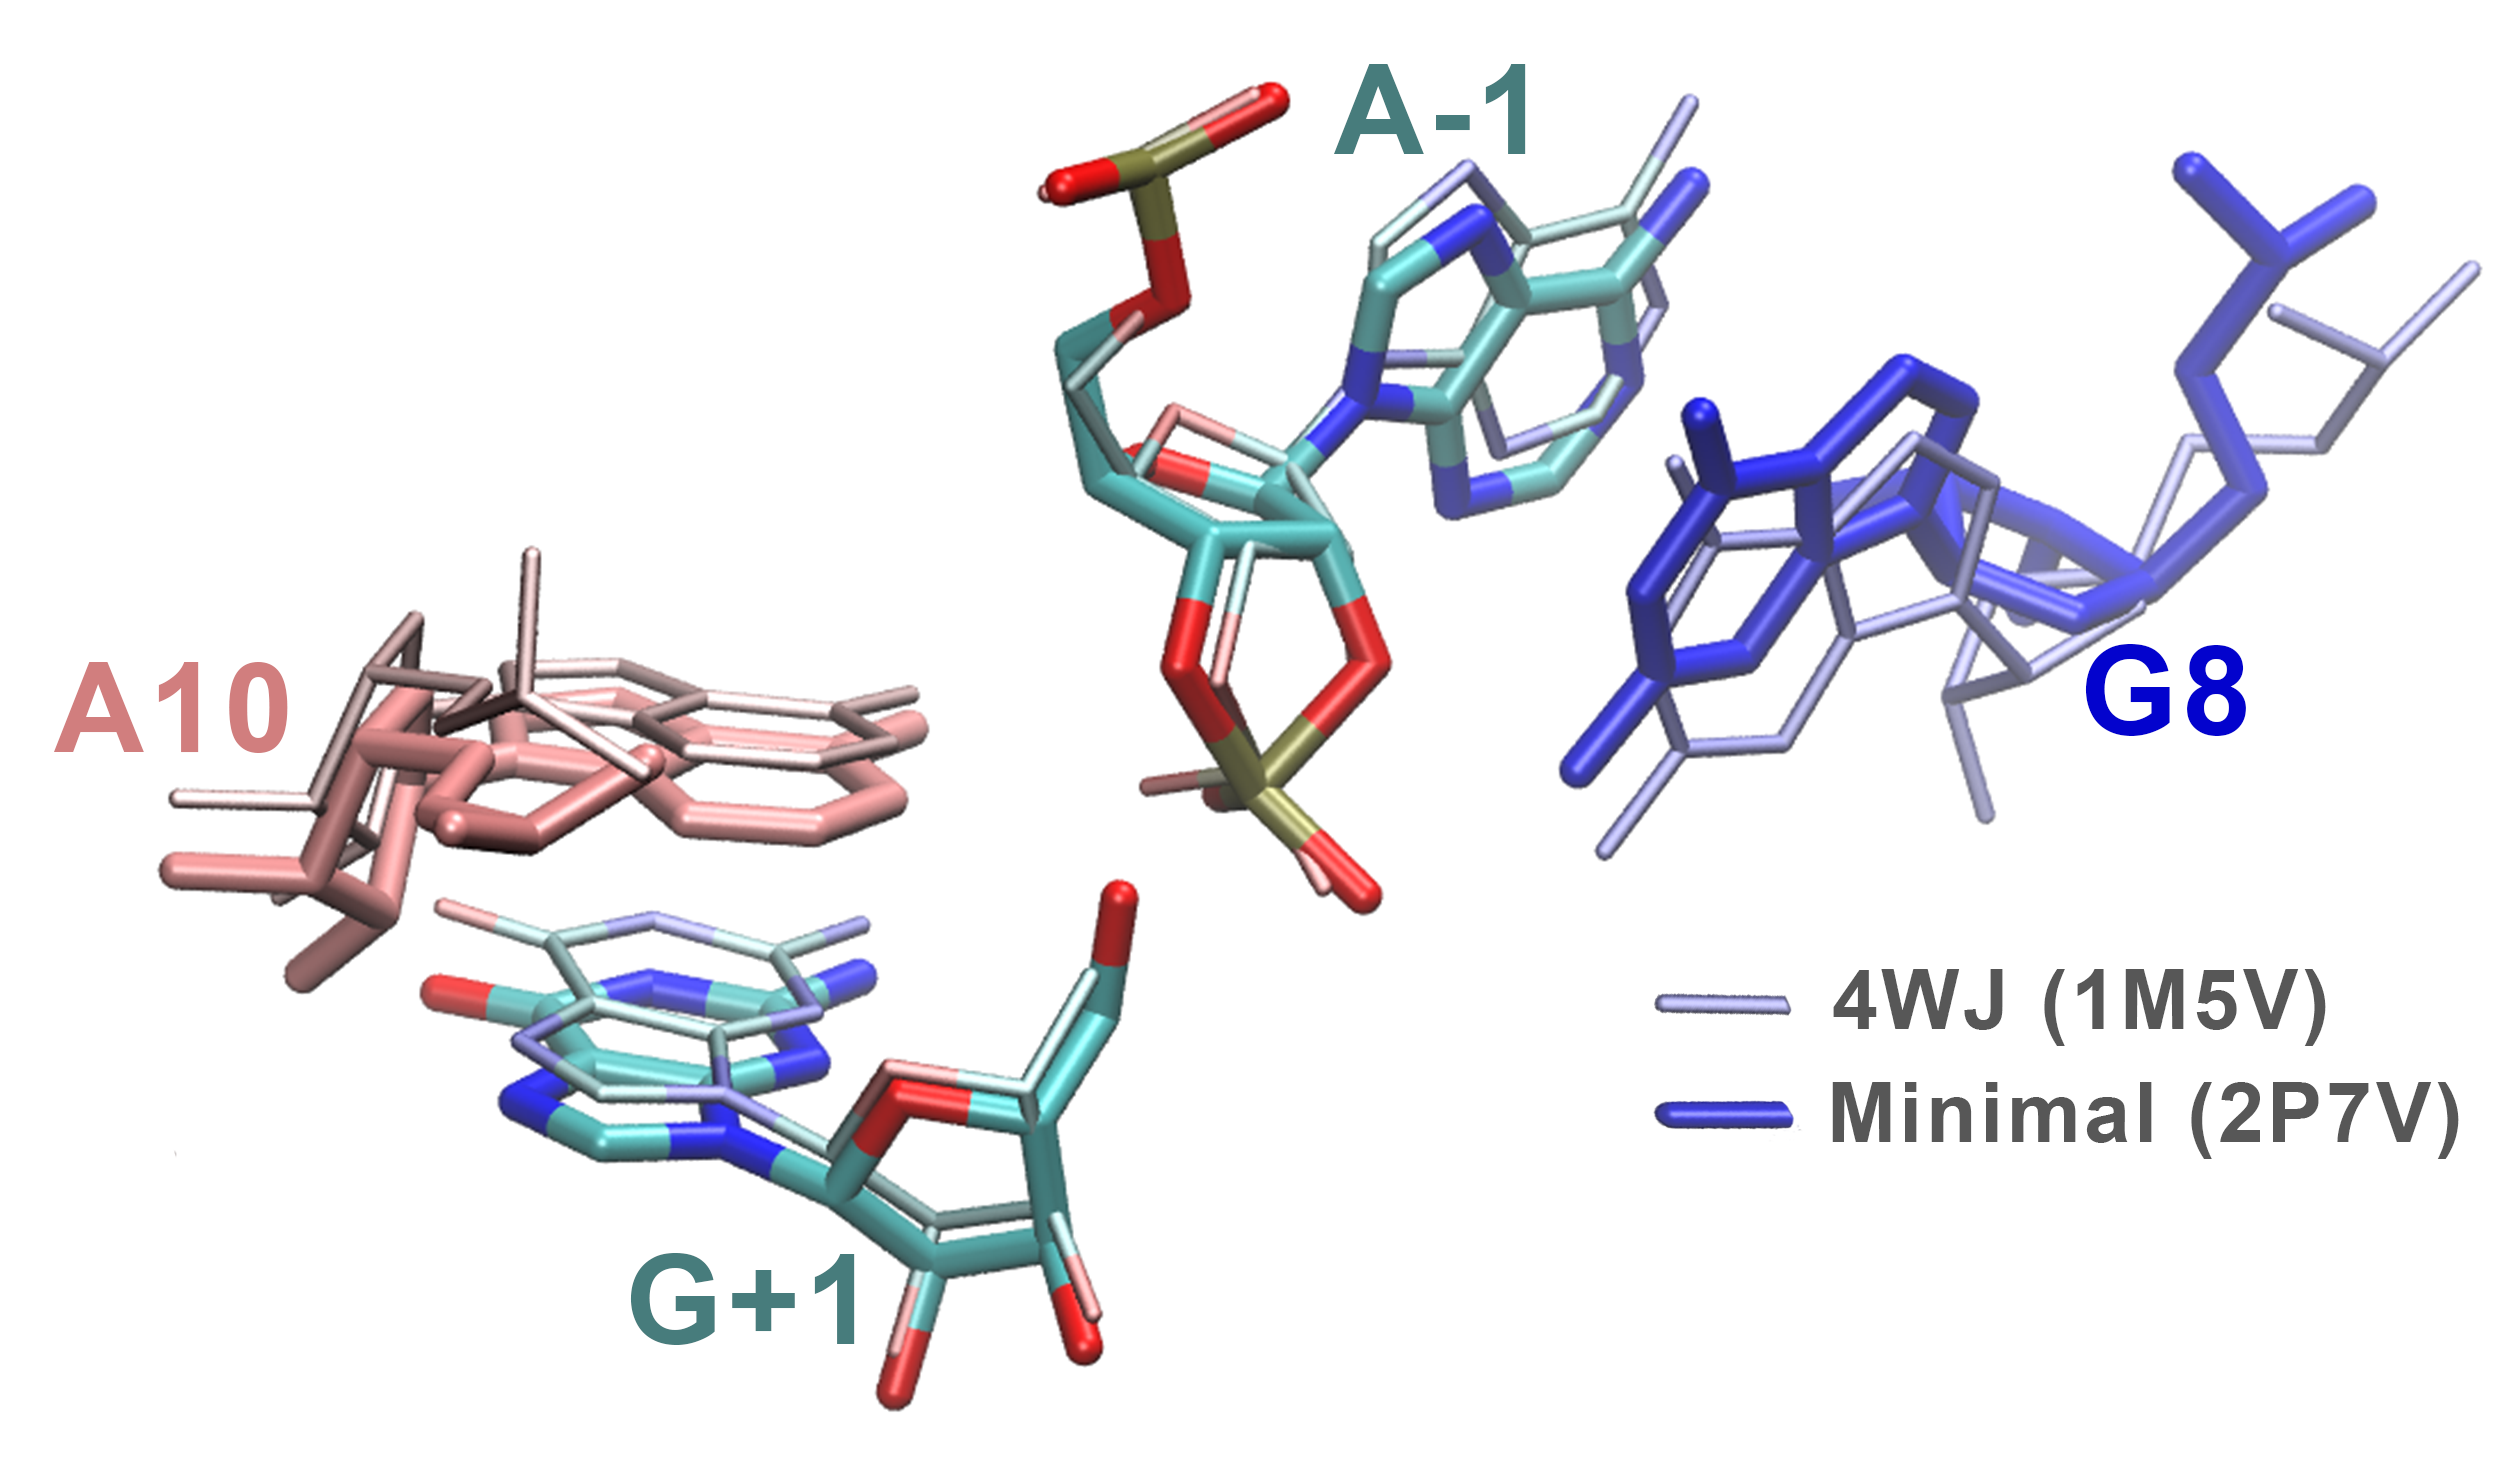
\includegraphics[width=0.8\textwidth]{figures_SI/Crystal_Cleaved_States.png}
    \caption[Comparison of the Cleaved States Crystal Structures]
    {Comparison of the Cleaved States Crystal Structures: 
    the 4WJ hairpin ribozyme (PDB ID: 1M5V) in light colors and thin representation, 
    the minimal hairpin ribozyme (PDB ID: 2P7D) used as initial structure for the cleaved states in this study is strong colors and thick representation.
    The two catalytic sites differ by only 0.93~\AA, calculated over all heavy atoms appearing here, 
    that is to say residues A-1, G+1, G8 and A38.}
    \label{fig:cleaved_crystals}
\end{figure}


% \begin{table}
% \caption{Summary of the non-standard residues of this chapter. 1. }
% \label{table:int_params}
% \begin{scriptsize}
% \begin{tabular}{c c c c c c}
% \hline
% & Name & Residue Type/Index & Scenario & Charge & Reference\\
% \hline
% \subf{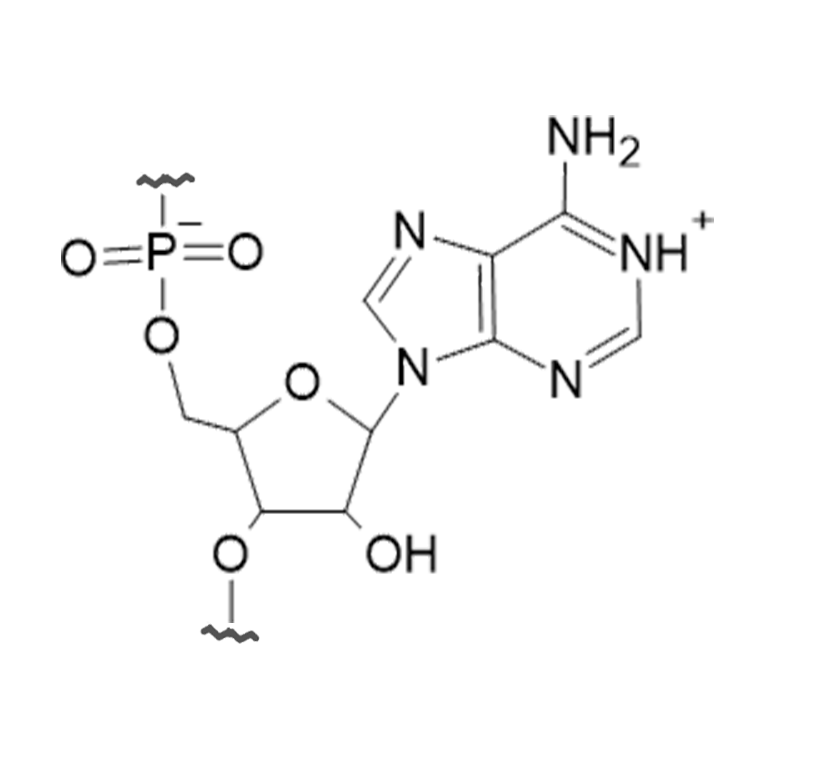
\includegraphics[width=30mm]{figures_SI/RAP_cut.png}}{} & RAP & A38 & All & 0 & available in \cite{mlynsky_extensive_2010} \\
% \subf{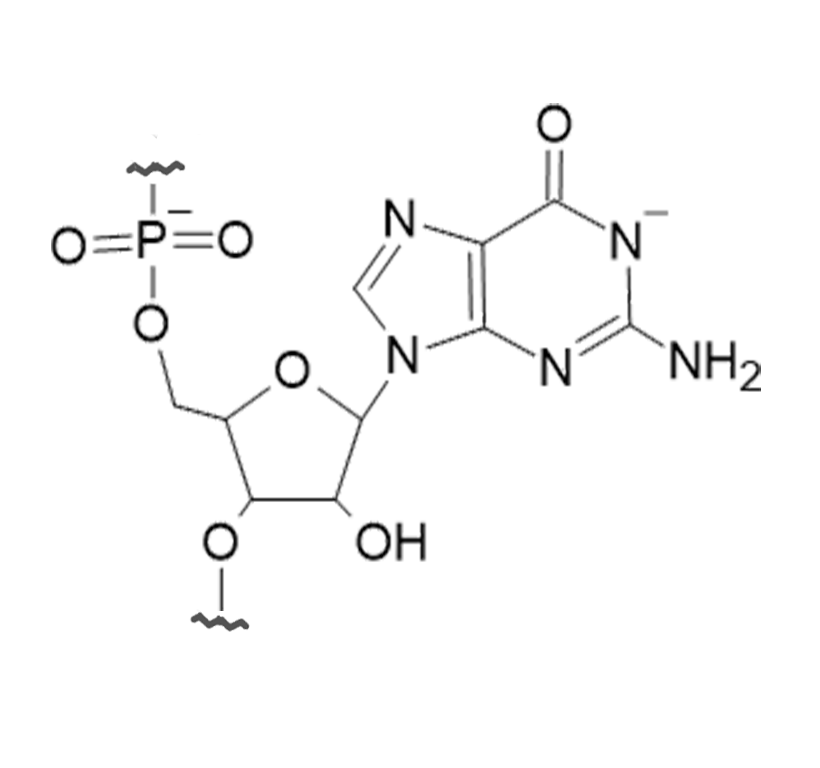
\includegraphics[width=30mm]{figures_SI/RGM_cut.png}}{} & RGM & G8 & Dianionic & -2 & adapted from \cite{mlynsky_extensive_2010} \\
% \subf{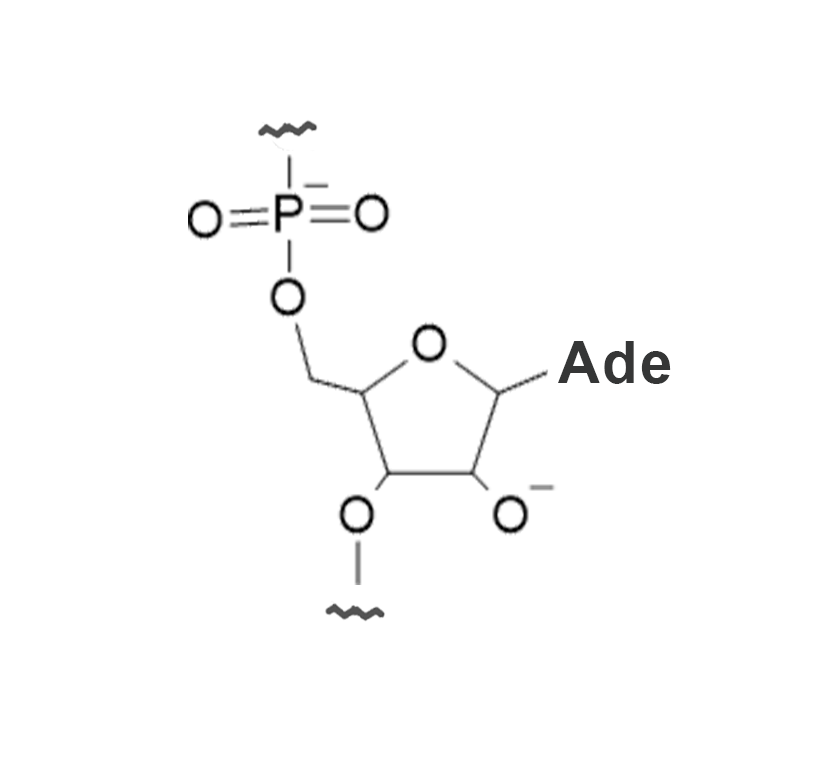
\includegraphics[width=30mm]{figures_SI/AD_cut.png}}{} & AD  & A-1 & Dianionic & -2 & / \\
% \subf{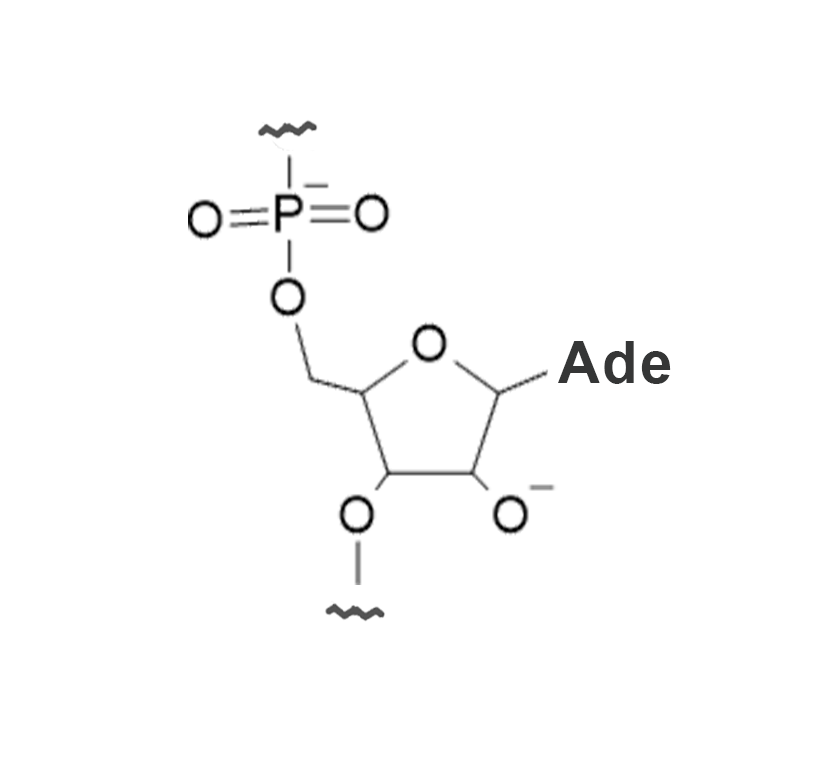
\includegraphics[width=30mm]{figures_SI/RAA_cut.png}}{} & RAA & A-1 & Mono-anionic & -2 & adapted from \cite{kumar_mechanistic_2018} \\
% \subf{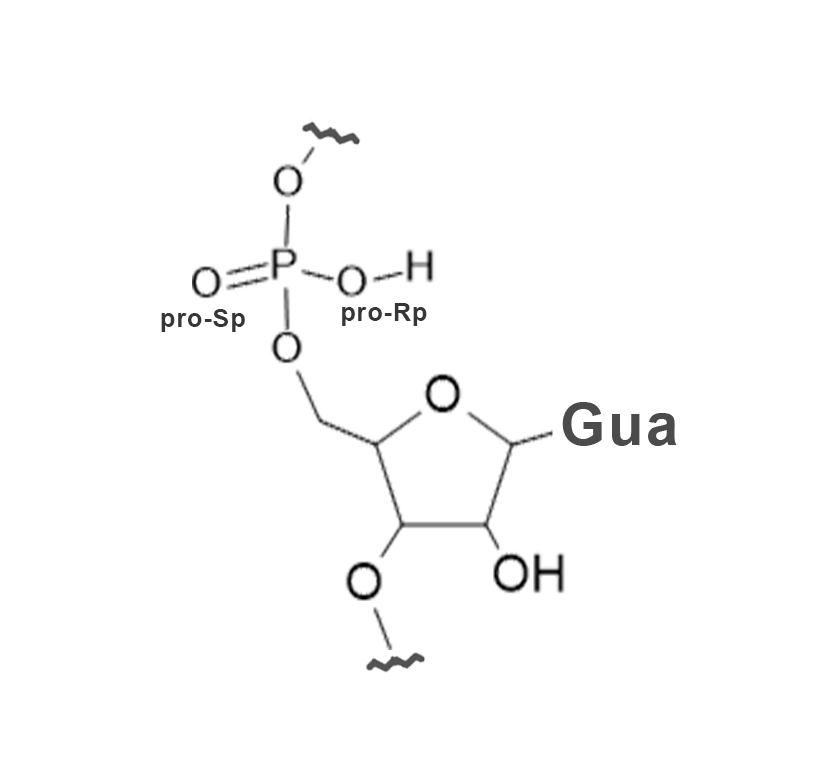
\includegraphics[width=30mm]{figures_SI/GAA_cut.png}}{} & GAA & G+1 & Mono-anionic & 0 & adapted from \cite{kumar_mechanistic_2018} \\
% \subf{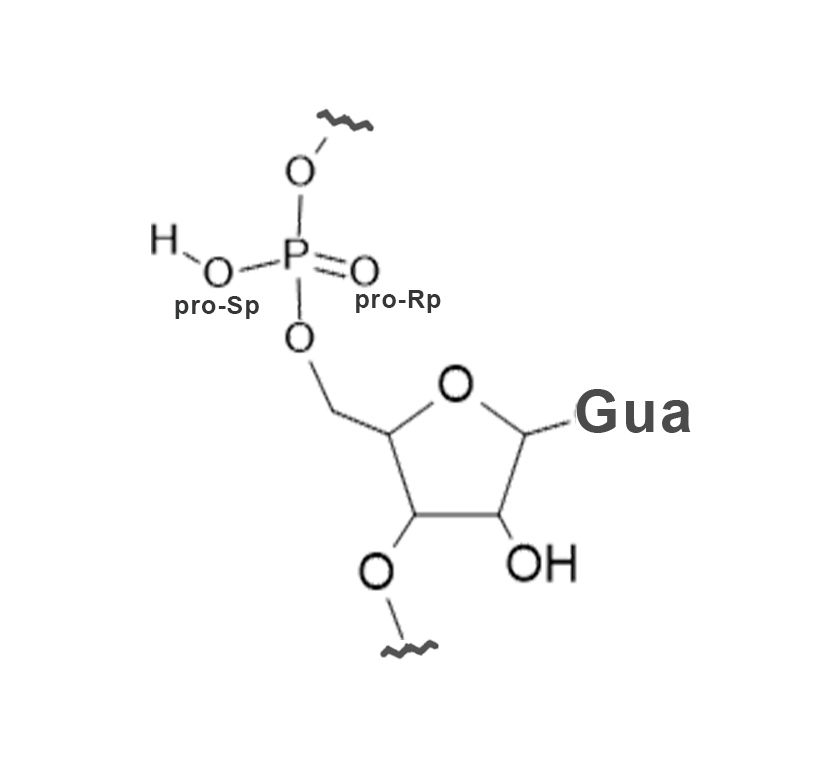
\includegraphics[width=30mm]{figures_SI/GSA_cut.png}}{} & GSA & G+1 & Mono-anionic & 0 & adapted from \cite{kumar_mechanistic_2018} \\
% \subf{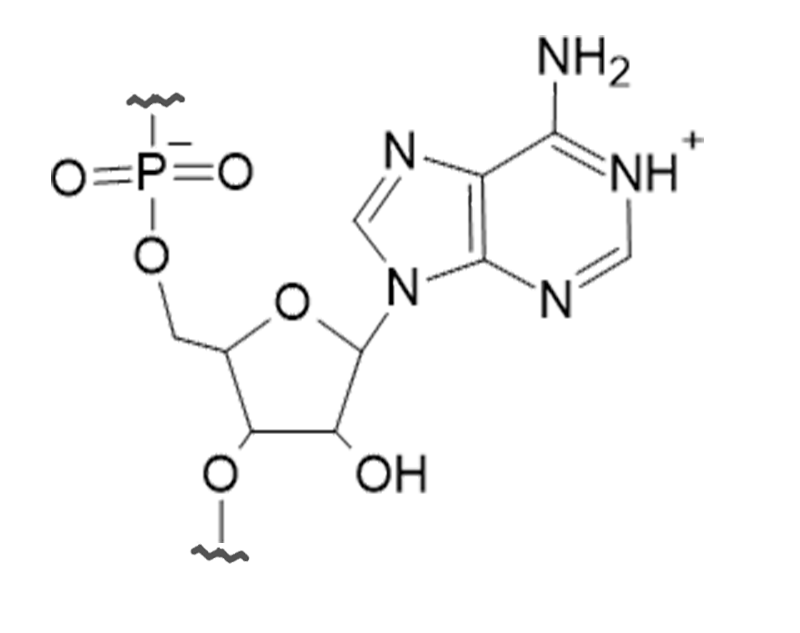
\includegraphics[width=30mm]{figures_SI/RAP_clean.png}}{} & RAC & A-1 & All & -1 & / \\

% \end{tabular}
% \end{scriptsize}
% \end{table}

\end{suppinfo}

%%%%%%%%%%%%%%%%%%%%%%%%%%%%%%%%%%%%%%%%%%%%%%%%%%%%%%%%%%%%%%%%%%%%%
%% The appropriate \bibliography command should be placed here.
%% Notice that the class file automatically sets \bibliographystyle
%% and also names the section correctly.
%%%%%%%%%%%%%%%%%%%%%%%%%%%%%%%%%%%%%%%%%%%%%%%%%%%%%%%%%%%%%%%%%%%%%
\bibliography{Thesis_v14_clean}

\end{document}